\documentclass[12pt]{article}
\usepackage[utf8]{inputenc}
\usepackage{geometry}
\usepackage{graphics}
\usepackage[T1]{fontenc}
\usepackage[french]{babel}
\usepackage{amsmath}
\usepackage{amssymb}
\usepackage{mathrsfs}
\usepackage{graphicx}
\usepackage{caption}
\usepackage{float}
\usepackage{amsfonts}
\usepackage{enumitem}
\usepackage{pifont}
\usepackage{array}
\usepackage{color}
\addto\captionsfrench{\def\tablename{TABLEAU}}
\geometry{hmargin=2cm,vmargin=2cm}

\begin{document}

\begin{titlepage}
\begin{center}

%\includegraphics[width=8cm]{Logo_EIRB.PNG}

\vspace{3cm}

\huge
\textbf{Résolution du système d'équations de Saint-Venant} \\
\vspace{0.7cm}
\Large
Compte Rendu\\
\ Travail en groupe \\
\large
\vspace{0.7cm}
M1 - EDPMA\\
Groupe AlMati\\
\vspace{0.7cm}
Alice \bsc{Castagnet} \\ Marine \bsc{Redondo} \\ Tiffanie \bsc{CARLIER} \\
\vspace{0.7cm}
Encadrant\\
\bsc{M. Leguèbe}\\
\vspace{2cm}
\Large
\textbf{14 novembre 2018}
\end{center}
\end{titlepage}

\normalsize

\newpage
\tableofcontents
\newpage
\section{Introduction}

\noindent Dans le cadre de l'approximation des grands lacs ( à détailler ?), les équations de Saint-Venant permettent de modéliser la hauteur et la quantité de mouvement des étendues d'eau pour calculer par exemple l'écoulement d'une rivière ou son débordement. 
\\
\\Ses équations s'écrivent sous la forme d'un système d'équations aux dérivées partielles non linéaire. Dans un premier temps, nous simplifierons le problème en nous intéressant à l'équation de transport scalaire :

\begin{center}
    $\partial_t u + div(cu) = 0 \text{ \: dans un ouvert } \Omega $
\end{center}

\noindent où $c$ est le champ de vecteur vitesse avec $div(c)=0$. 
\\
\\La méthode des volumes finis est la plus adaptée à ce type d'équation. Notre objectif est donc de résoudre une rupture de barrage pour les équations de Saint-Venant \cite{ref1} en utilisant la méthode des volumes finis.


\section{Notations}

\noindent $\Omega$ : ensemble d'espace associé au problème
\\$u$ : inconnue du problème
\\$t$ : variable de temps
\\$\Delta t$ : pas de temps
\\$n$ : nombre d'itérations en temps
\\$x$ : variable d'espace qui peut avoir plusieurs dimensions
\\$\Delta x$ : pas d'espace en une dimension
\\$i$ : nombre d'itérations en espace
\\$c$ : vitesse de $u$
\\$K_i$ : volumes de contrôle où $K_i$ et $K_j$ sont deux volumes côte à côte
\\$e$ : arête quelconque
\\$\epsilon K_i$ : ensemble des arêtes du volume de contrôle $K_i$
\\$e_{i,j}$ : arête commune aux volumes $K_i$ et $K_j$
\\$n_{i,j}$ : normale à l'arête $e_{i,j}$ extérieure à $K_i$

	
\section{Recherche de ressources, documentation}
\subsection{L'équation de transport}
\noindent 1. Une équation de transport est une équation de la forme :

\begin{center}
    $\partial_tu(t,x)+c(t,x,u).\nabla_xu(t,x)=0 $
\end{center}

\noindent Elle décrit le comportement d'une quantité $u$ dépendant du temps $t$ et d'une autre variable $x$ appartenant à un domaine $\Omega$ qui représente généralement un ouvert régulier de $\mathbb{R}^n$. La variable $x$ peut définir une position, une vitesse, un couple position/vitesse... 
\newpage \noindent Les équations de transport font apparaître une notion de propagation à vitesse finie et sont donc qualifiées d'équations d'hyperboliques.
\\
\\Il en existe deux formes : 
\\
\\- la forme conservative :

\begin{eqnarray*}
\left\{ 
    \begin{array}{llll}
        u_t(t,x)+div_x(c(t,x)u(t,x))=0
        \\u(t=0,x)=u_0(x)
       	\end{array}
    \right .
\end{eqnarray*}
\\
\\
- la forme forte : 

\begin{eqnarray*}
\left\{ 
    \begin{array}{llll}
        u_t(t,x)+c(t,x)\nabla_xu(t,x)=d(t,x,u)
        \\u(t=0,x)=u_0(x)
       	\end{array}
    \right .
\end{eqnarray*}
\\
\\
\noindent Dans notre cas, nous utiliserons la forme conservative de l'équation de transport car la divergence du vecteur vitesse $c$ sera nulle. Ceci nous permet ainsi de dire que l'intégrale de $u$ sera conservée au cours du temps. 
\\
\\Pour résoudre le problème, il est nécessaire d'imposer une condition initiale à $t=0$ : \\$u(t=0,x)=u_0(x)$.
\\De plus, si $\Omega$ possède des bords il faut pour que le problème soit bien posé, ajouter  une condition $u_{b}$ sur la partie de la frontière où le champ est rentrant, c'est-à-dire :
\\
\begin{center}
$\forall t\in \mathbb{R}_{+}, \forall x\in \partial\Omega,\;\;c(t,x).\overrightarrow{n(x)}\,<\,0\; \Rightarrow\, u(t,x) = u_b(t,x)$
\end{center}
où $\overrightarrow{n(x)}$ représente la normale extérieure à $\Omega$.
\\Ceci permet d'éviter au problème d'être sur-déterminé et de vérifier ainsi les trois conditions nécessaires qui définissent un problème bien posé (existence, unicité et stabilité).
\\ 
\\Dans le cas 1D où $x\in (0,1)$ et $t\in (0,T)$ que l'on étudiera par la suite, les conditions aux limites se présentent de cette manière :
\\
Si $c>0$ alors il est nécessaire d'ajouter sur le bord gauche qui est entrant la condition suivante : $u(0,t)=g_0(t)$
\\ Au contraire si $c<0$ alors il est nécessaire d'ajouter sur le bord droit la condition suivante : $u(1,t)=g_1(t)$ 
\\
\subsection{Résolution du problème 1D}
\subsubsection{Résolution par la méthode des caractéristiques}
Dans le cas 1D avec un champ de vitesse constant $c$ le problème s'écrit sous la forme :
\begin{eqnarray*}
    \left\{ 
    \begin{array}{llll}
        \partial_tu(t,x) + c\partial_xu(t,x)=0, x \in \mathbb{R} \text{ et } t \in (0,T)
        \\u(0,x)=u_0(x)
        \end{array}
    \right .
\end{eqnarray*}
\\
Une des méthodes pour résoudre ce type d'équation est la méthode des caractéristiques \cite{ref10}. On définit les caractéristiques comme les courbes de $\mathbb{R}^2$ définies par $(t,X(t))$ où $X(t)$ est la solution de l'équation différentielle ordinaire $\partial_tX(t)=c$.
On a alors que $(t,X(t))$ vérifie :
\\
\begin{center}
        $\partial_tu(t,X(t))=\partial_tX.\partial_xu+\partial_tu
        =c.\partial_xu+\partial_tu =0$
\end{center}
Les solutions sont donc constantes le long des caractéristiques. 
Considérons $(t^*,x^*)$ un point du plan avec $t^*>0$ ainsi que $X^*(t)$ la caractéristique passant par ce point. Alors $X^*$ vérifie :

\begin{center}
        $\partial_tX^*=c \;,\;  X^*(t^*)=x^*
        \Rightarrow\ X^*=ct+x^*-ct^*\; \text{et donc } X^*(0)=x*-ct^*$
\end{center}

\noindent Finalement au point $(t^*,x^*)$ sachant que la variable $t$ ne rentre pas en compte car $u$ est constante le long des caractéristiques, la solution $u$ du problème est déterminée par :

\begin{center}
    $u(t^*,x^*)=u(0,X^*(0))=u(0,x^*-ct^*)=u_0(x^*-ct^*)$
\end{center}

\noindent On obtient finalement le critère suivant :
\\ Si $u_0$ est dérivable sur $\mathbb{R}$, alors il existe pour le problème de transport en une dimension une unique solution différentiable $u$ en $(t,x)$  donnée par :

\begin{center}
        $u(t,x)=u_0(x-ct) \;\;\;\;\forall x\in \mathbb{R}, \forall t>0 $
\end{center}
 Cela signifie que connaissant $u_0(x_0)$ on peut déterminer u(x,t) sur toute la demi droite caractéristique issue de $x_0$ pour tout $x_0$
\\
\begin{figure}[H]
	\centering
	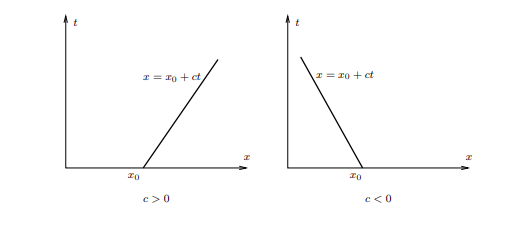
\includegraphics[scale=1]{dr.png}
	\caption{Direction des caractéristiques suivant la valeur de $c$}
	\label{1D}
	\end{figure}
\newpage
\subsubsection{Application}
Considérons l'exemple d'un tube dans lequel coule de l'eau à une vitesse $c$ que l'on choisit positive telle que l'eau présente des traces d'un certain polluant. Ainsi d'après ce que l'on a prouvé précédemment, la distribution du polluant à l'instant $t=0$ est inchangée pour un temps $t_1 > 0$ à une translation près de $ct_1$.
\\
\\\begin{figure}[H]
	\centering
	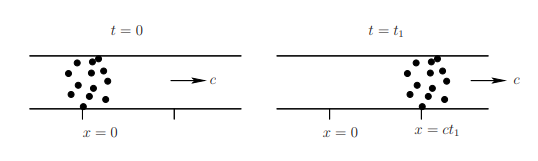
\includegraphics[scale=1]{transport_de_polluant.png}
	\caption{Transport d'un polluant}
	\label{1D}
	\end{figure}
	
	
\subsection{Méthodes des volumes finis}

\subsubsection{Notion de maillage et de discrétisation}

\noindent Pour définir la méthode des volumes finis il est nécessaire de définir la notion de maillage.
Un maillage est la discrétisation spatiale d'un milieu continu, ou une modélisation géométrique d'un domaine par des éléments proportionnés finis et bien définis. Un maillage doit vérifier les propriétés suivantes :
\\Soit $\Omega$ l'ensemble d'espace associé à notre problème. 
Les éléments de la suite $(K_i)_{1\leq{i}\leq{I}}$ sont appelés volumes de contrôle. Cette suite définie un maillage du domaine $\Omega$  vérifiant :
\\  $K_i$ un ouvert de $\Omega$
\\  $K_i \cap K_j = \varnothing, \forall i \neq j$
\\  $\cup_{i=1}^{I} \overline{K_i} = \overline{\Omega}$

\noindent En voici un exemple dans le cas d'un maillage "cell vertex" :

    \begin{figure}[H]
	\centering
	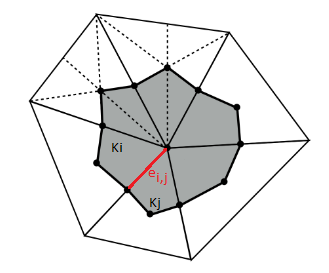
\includegraphics[scale=0.5]{Ki.png}
	\caption{Exemple d'un ensemble d'espace $\Omega$ divisé en espaces de contrôle $K_i$}
	\label{Ki}
	\end{figure}
\newpage
\subsubsection{Volumes finis en dimension quelconque}
\noindent En considérant un maillage défini comme précédemment, le principe des volumes finis \cite{ref7} est l'intégration de l'équation aux dérivées partielles donc dans notre cas l'équation de transport sur tous les volumes de contrôle. 
La formule de la divergence nous permet de simplifier le problème qui nous dit :
\\
\begin{center}
    $\displaystyle\int\limits_{K} div\, w \; dK=\int\limits_{\partial{K}} w.n \; d(\partial{K}) = \displaystyle\sum_{\sigma \in \varepsilon{K}} \int_{\sigma} \omega_{\sigma}.n_{\sigma} \; d\gamma$
\end{center}
où $\varepsilon K$ est l'ensemble des arêtes du volume de contrôle $K$, $n_{\sigma}$ est la normale à l'extérieur par rapport à l'arête $\sigma$, et $\gamma$ la mesure sur $\sigma$.
\\
\\Ainsi, pour l'équation de transport la méthode des volumes finis donne sur un volume de contrôle $K_i$ :

\begin{eqnarray}
       \frac{d}{dt} \int\limits_{K_i} u(t,x)dx + \displaystyle \sum_{e_{i,j}\in \partial K_i} \int_{e_{i,j}} (cu).{n_{i,j}} \; d\gamma=0
       \\mes(K_i)\frac{d\,u_i}{dt}=-\displaystyle\sum_{e_{i,j}\in \partial K_i} \int_{e_{i,j}} (cu).{n_{i,j}} \; d\gamma
\end{eqnarray}

\noindent Ici, $\gamma$ est la mesure de $e_{i,j}$ où $e_{i,j}$ est l'arête commune aux deux volumes de contrôle $K_i$ et $K_j$ et $n_{i,j}$ est la normale à l'arête $e_{i,j}$ sortant du volume de contrôle $K_i$. 
\textcolor{red}{Ajouter Figure ?}

\subsubsection{Méthode des volumes finis cas 1D }
\paragraph{Méthode générale :}
La Figure ci-dessous représente un maillage en 1 dimension. Ici, l'espace $\Omega$ est le segment $[AB]$. On divise ce segment en petits segments délimités par les points $x_i$ où $i\in \{1,l\}$ (en vert sur le schéma). On note que ici, tous les $x_i$ sont strictement à l'intérieur des extrémités $A$ et $B$, le volume de contrôle devant être ouvert. On définit ensuite les $x_{i\pm\frac{1}{2}}$ (en rouge sur le schéma). Les volumes de contrôle $K_i$ définis précédemment correspondent aux intervalles ouverts $]x_{i-\frac{1}{2}},x_{i+\frac{1}{2}}[$ pour $i\in \{1,l\}$.
\\Dans le cas ci-dessous, les $x_i$ sont situés au milieu de $K_i$ mais il est également possible de choisir les $x_i$ à l'une ou l'autre des extrémités des $K_i$. 

    \begin{figure}[H]
	\centering
	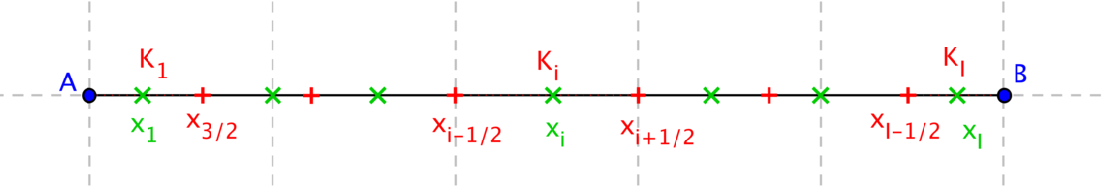
\includegraphics[scale=0.4]{VF2.png}
	\caption{Maillage en 1 dimension}
	\label{1D}
	\end{figure}
\newpage
\noindent Pour calculer numériquement la solution du problème 1D on introduit une grille qui est cette fois en x et en t.
\noindent On introduit les notations suivantes :
\\
 $x_i=i\Delta x, \Delta x$ le pas de la discrétisation en espace
\\
$ t^n=n\Delta t, \Delta t$ le pas de la discrétisation en temps
\\De plus on note $u_i^n$ une approximation de $u(x_i,t^n)$
 \begin{figure}[H]
	\centering
	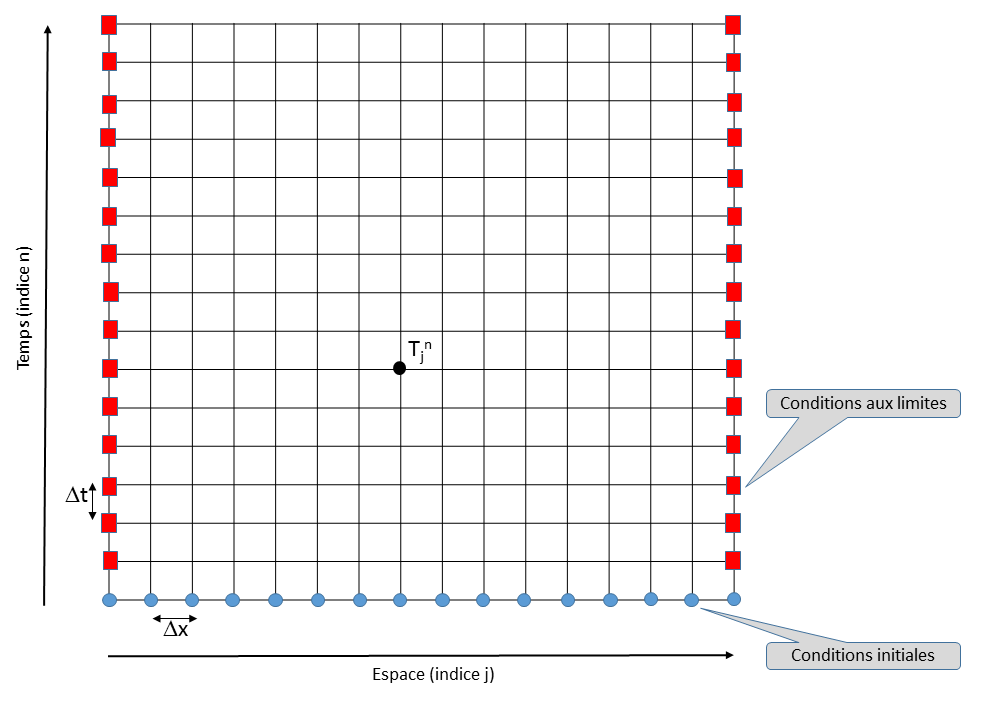
\includegraphics[scale=0.3]{DFGrille.PNG}
	\caption{Grille de la discrétisation}
	\label{1D}
	\end{figure}
\noindent On intègre l’équation de transport sur tous les volumes de contrôle donc ici sur une dimension d'espace et sur la discrétisation en temps que l'on a défini précédemment, cela nous donne :

\begin{center}
      $ \displaystyle \int_{t}^{t+\partial t}\int_{x_{i-\frac{1}{2}}}^{x_{i+\frac{1}{2}}}\partial_tu(t,x) dxdt + \int_{n\partial t}^{(n+1)\partial t}\int_{x_{i-\frac{1}{2}}}^{x_{i+\frac{1}{2}}} \partial_xu(t,x) dxdt =0$
      \\$\Leftrightarrow \displaystyle \partial_x (u_k^{n+1} -u_k^n) + c\partial_t \left(u_{k+\frac{1}{2}}^{n+\frac{1}{2}}-u_{k-\frac{1}{2}}^{n+\frac{1}{2}}\right)=0$
\end{center}
\noindent Comme dit précédemment, la méthode des volumes finis consiste à intégrer le problème que l'on cherche à résoudre sur les différents volumes de contrôle. Ceci nous permet ainsi d'obtenir autant d'équations que de volumes de contrôles. 

\subsubsection{Exemples de schémas numériques dans le cas 1D}

\noindent Il est alors possible grâce par exemple au schéma d'Euler explicite d'obtenir un schéma "Volumes Finis".
La méthode d'Euler pour un schéma explicite consiste à associer à une équation différentielle du type :
\begin{center}
        $\partial u_t(t,x)=f(t,x)$
\end{center}
à un schéma avec un pas de temps $\Delta t$ donné par :
\begin{eqnarray}
        u^{n+1}-u^{n} =  \int_{t^{n}}^{t^{n+1}}\big(f(s,u(s)))ds
\end{eqnarray}

\newpage \noindent En appliquant la méthode d'Euler à l'équation (3), on obtient :

\begin{center}
        $u^{n+1}_i=u_i^n + \displaystyle c \, \frac{\Delta t}{\Delta x}(u_{i+\frac{1}{2}}^n-u_{i-\frac{1}{2}}^n)$
        \leavevmode\\
        \leavevmode\\
        $u^{n+1}_i=u_i^n +  \displaystyle c \, \frac{\Delta t}{\Delta x}\left(\frac{u_{i+1}^n-u_{i-1}^n}{2}\right)$
\end{center}

\noindent où $u_{i+\frac{1}{2}} = \displaystyle\frac{u_i+u_{i+1}}{2}$ \: et \: $u_{i-\frac{1}{2}} = \displaystyle\frac{u_{i-1}-u_{i}}{2}$.
\\
\\
Il s'agit ici du schéma centré de Richardson. Malheureusement, ce schéma est instable car il ne prend pas en compte l'information sur le signe du champ de vecteur vitesse $c$. Pour le rendre stable, il faudrait apporter de la diffusion numérique.
D'autres schémas existent, quelques uns sont listés ci-dessous \cite{ref11}.
\\
\\- Les schémas décentrés (upwind)
\begin{eqnarray*}
        u^{n+1}_i=u_i^n-\frac{c\Delta t}{\Delta x}({u_{i}^n-u_{i-1}^n}) \text{       , si c>0}
        \iff u^{n+1}_i=u_i^n\left(1-\frac{c\Delta t}{\Delta x}\right)+u_{i-1}^n\left(\frac{c\Delta t}{\Delta x}\right)	
        \\
        \\
        u^{n+1}_i=u_i^n-\frac{c\Delta t}{\Delta x}({u_{i+1}^n-u_{i}^n}) \text{       , si c<0}
        \iff u^{n+1}_i=u_i^n\left(1+\frac{c\Delta t}{\Delta x}\right)-u_{i+1}^n\left(\frac{c\Delta t}{\Delta x}\right)
\end{eqnarray*}

\noindent Il s'agit ici d'un schéma décentré permettant de prendre l'information du bon côté suivant la direction de la caractéristique donné par le signe du champ vitesse $c$ i.e que le décentrement tient compte de la direction de la propagation.
\\On constatera par la suite qu'il s'agit du meilleur schéma dans le cas 1D tel que la convergence soit assurée peu importe la valeur du vecteur c. Il est tout de même important de préciser que la condition de CFL inférieure ou égale à 1 est toujours une obligation.
L'ordre global avec ce schéma est en $O(\delta t + \delta x)$.
\\
\\- Le schéma de Lax-Wendroff :
\\
\begin{eqnarray*}
        u^{n+1}_i=u_i^n-\frac{c\Delta t}{\Delta x}({u_{i+1}^n-u_{i-1}^n}) +\frac{c^2\Delta t^2}{\Delta x^2}(u_{i+1}^n-2u_{i}^n+u^{n}_{i-1})
\end{eqnarray*}
\\
La condition de CFL 
\\- Le schéma Euler explicite en aval :
\\
\begin{eqnarray*}
        u^{n+1}_i=u_i^n-\frac{c\Delta t}{\Delta x}({u_{i+1}^n-u_{i}^n})
\end{eqnarray*}

\newpage
\subsection{Flux numérique}
\subsubsection{La mécanique des fluides}
\noindent La mécanique des fluides numériques est l'étude des mouvements d'un fluide par la résolution numérique des équations décrivant le comportement du fluide. Il s'agit d'un outil essentiel dans de nombreuses branches de la dynamique des fluides : propulsion aérospatiale, météorologie, barrage hydraulique, écoulement d'un fluide dans un tuyau... L'avantage de cette approche est qu'elle donne accès à toutes les informations instantanées (vitesse, pression, concentration...) en chaque point du domaine de calcul, pour un faible coût par rapport aux expériences correspondantes. 
\\
\\La résolution d'un problème de mécanique des fluides numériques comprend trois étapes :
\\- l'analyse du problème : choix d'une géométrie, d'un maillage discrétisant le domaine de calcul, des méthodes numériques employées ;
\\- la résolution numérique du problème : exécution d'un programme informatique ;
\\- l'exploitation des résultats : vérification de la cohérence puis étude des résultats.
\\
\\Les trois méthodes de discrétisation sont :
\\- méthode des différences finies
\\- méthode des volumes finis
\\- méthode des éléments finis
\\Cependant, c'est la méthode des volumes finis qui est la plus appropriée et la plus utilisée pour résoudre des problèmes de dynamique des fluides.
La méthode des volumes finis est complètement déterminée par son flux numérique.
\\

\noindent Dans notre cas le flux numérique vérifie deux propriétés :
\\- la conservation des flux à travers les arêtes
\\ - la consistance des flux
\\
\subsubsection{Exemple de flux numérique}
\noindent Prenons le problème suivant :
\begin{eqnarray*}
        -u''(x)=f(x) ,  x\in]0,1[
        \\u(0)=u(1)=0
\end{eqnarray*}
En appliquant la méthode des volumes finis à cette équation on obtient le schéma suivant :
\begin{eqnarray*}
        -u'(x_{i+\frac{1}{2}})+u'(x_{i-\frac{1}{2}})=h_if_i
        \\
        \\
        \Leftrightarrow F_{i+\frac{1}{2}} -F_{i-\frac{1}{2}} = h_if_i
\end{eqnarray*}
$F_{i+\frac{1}{2}}$ est appelé le flux numérique en $x_{i+\frac{1}{2}}$.
\\
Un des principes de la méthode des volumes finis est de pouvoir écrire les flux numériques en fonction des variables discrètes $u_i$.
Une approximation de ce flux numérique peut alors être donnée par la notation suivante :
\\
\begin{eqnarray*}
        F_{i+\frac{1}{2}} = -\frac{u_{i+1}-u_i}{h_{i+\frac{1}{2}}}
\end{eqnarray*}
\\
En ce qui concerne le cas général on peut définir le flux comme suivant :
le flux à travers l'arête $e_{i,j}$ est approché par 
\begin{eqnarray*}
       \int_{e_{i,j}} (cu).{n_{i,j}} \; d\gamma=mes(e_{i,j})\Phi(u_i,u_j,n_{i,j})
\end{eqnarray*}

\noindent où $\Phi(u_i,u_j,n_{i,j})$ est le flux numérique à travers l'arête $e_{i,j}$ entre les volumes de contrôle $K_i$ et $K_j$ définit ainsi :

\begin{eqnarray*}
       \Phi(u_i,u_j,n_{i,j})=
        \left\{ 
        \begin{array}{llll}
            u_{K_i}(\bar c.n_{i,j}) \text{ si }\bar c.n_{i,j}> 0 
            \\u_{K_j}(\bar c.n_{i,j}) \text{ sinon}
        \end{array}
    \right .
    \\
    \\
    = u_{K_i}(\bar c.n_{i,j})^+ + u_{K_j}(\bar c.n_{i,j})^-
\end{eqnarray*}

\noindent où $(\bar c.n_e)^+=\text{max}(\bar c.n_e,0)$, \, $(\bar c.n_e)^-=\text{min}(\bar c.n_e,0)$ \, et \, $\bar c$ \, est la moyenne de la vitesse $c$ aux extrémités $x_1$ et $x_2$ de l'arête $e$ :

\begin{eqnarray*}
       \bar c=\frac{c(x_1)+c(x_2)}{2}
\end{eqnarray*}

\noindent On utilise donc l'information venant des espaces de contrôle $K_i$ ou $K_j$ en fonction de la direction du champ de vitesse $c$.

\subsubsection{Schéma numérique général}
\noindent En appliquant le schéma d'Euler \cite{ref6} à l'équation (2), on obtient un schéma dans le cas général donné par :
\begin{center}
       $\displaystyle \frac{d u_i}{dt}=-\frac{1}{mes(K_i)} \displaystyle\sum_{e_{i,j} \in \partial K_i} mes(e_{i,j})\Phi(u_i,u_j,n_{i,j})$
       \\
       $u_i^{n+1}=u_i^n-\frac{\Delta t}{mes(K_i)} \displaystyle\sum_{e_{i,j}\in \partial K_i} mes(e_{i,j}) (u_{K_i}(\bar c.n_{i,j})^+ + u_{K_j}(\bar c.n_{i,j})^-)$
\end{center}
 
 \subsection{Contraintes sur la méthode}
 \subsubsection{Condition de CFL et pas de temps}
\noindent Dans le cas 1D, pour écrire un schéma pertinent il faut que le pas de temps $\Delta t$ soit suffisamment petit pour que le pied de la caractéristique rentre dans le support du schéma, c'est une condition géométrique nécessaire à sa stabilité.
 \\Cela revient à dire que l'on cherche à avoir $\Delta t$ tel que le cône de dépendance théorique soit inclus dans le cône de dépendance numérique.
 
 \begin{figure}[H]
	\centering
	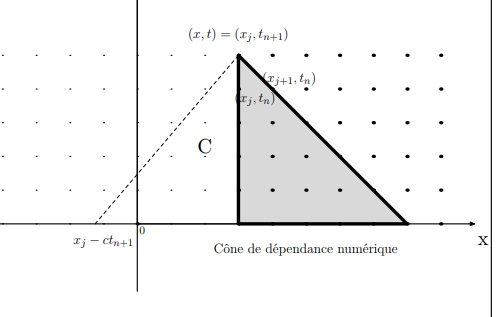
\includegraphics[scale=0.7]{cone.png}
	\caption{Exemple de cône de dépendance}
	\label{1D}
	\end{figure}
	
\noindent Numériquement et peu importe la dimension du problème, cette condition est équivalente à la condition de CFL \cite{ref9} (coefficient de Courant, Fredrichs, Lewy).
Le schéma est stable si ce coefficient est inférieur ou égal à 1 et produira une solution cohérente. 
La condition de CFL impose au coefficient d'amplification d'être plus petit que $1$.
\\Par exemple sur les schémas à un pas, un schéma numérique est déterminé par la formule suivante :

\begin{eqnarray*}
    \sum_{j\in J_k} b_ju_{k+j}^{n+1} = \sum_{j\in J_k} c_ju_{k+j}^{n} 
\end{eqnarray*}
\\Par passage à la transformée de Fourier, on exprime le coefficient d'amplification du schéma par :
\begin{eqnarray*}
     M(\xi)=\frac{\sum_j c_j e^{i\xi j \Delta_x}}{\sum_j b_j e^{i \xi j\Delta_x }}
\end{eqnarray*}
\\Ainsi lorsque que $|M(\xi)|\leq 1$ cela nous donne la condition de stabilité que l'on appelle CFL.
\\
\\
On peut déterminer par exemple le pas de temps avec la formule suivante :
$\Delta t = \Delta x \times CFL$
\\ou on fixe au préalable $CFL < 1$ et un pas d'espace $\Delta x$.
\\On peut parfois se placer à la condition de stabilité où le coefficient de $CFL$ vaut 1.
\\
\subsubsection{Méthode avec résolution de système linéaire}\noindent En fonction du type de schéma considéré pour l'approximation de l'équation,  c'est-à-dire si un schéma est implicite ou explicite on peut avoir besoin de résoudre un système linéaire. C'est dans le cas où le schéma est implicite c'est-à-dire lorsqu'au $n+1^{ième}$ pas de temps, il existe plusieurs pas d'espace pour ce même pas de temps, qu'il sera alors nécessaire de résoudre un système linéaire.
Les schémas implicites peuvent parfois être utilisés à la place des schémas explicites pour leur meilleure stabilité. 
Mais dans le cas où le schéma choisi est explicite, on peut calculer explicitement $u_k^n$ en fonction des $u_{k+1}^{n}$ ou des pas précédents sans avoir à résoudre un système linéaire.

\noindent Pour obtenir un schéma implicite on peut pour cela changer la discrétisation de l'élément $\partial_x$ en le discrétisant au pas de temps n+1. 
Un résultat possible est alors le schéma suivant :
\begin{eqnarray*}
         u_k^{n+1} +\frac{c\Delta t}{\Delta x}u_k^{n+1}-\frac{c\Delta t}{\Delta x}u_{k-1}^{n+1}=u_k^n
\end{eqnarray*}
\\Matriciellement celà vient à résoudre le système :
\begin{eqnarray*}
        \begin{pmatrix}
   1 & 0 & .. & .. &.. & 0 \\
   \frac{-c\Delta t}{\Delta x} & 1 + \frac{c\Delta t}{\Delta x} &0 &..&.. &0 \\
   0 & \frac{-c\Delta t}{\Delta x} & 1 + \frac{c\Delta t}{\Delta x} & 0 &.. & : \\
   : & 0 & . &  &.. & : \\
   : &  & . &  &.. & 0 \\
   0 & . & . & 0 &\frac{-c\Delta t}{\Delta x} & 1 + \frac{c\Delta t}{\Delta x}
   
\end{pmatrix}
*         \begin{pmatrix}
  u_0\\
  u_1\\
  ..\\
  ..\\
  u_{n-1}\\
  u_n
\end{pmatrix}^{n+1}
= \begin{pmatrix}
  u_0\\
  u_1\\
  ..\\
  ..\\
  u_{n-1}\\
  u_n
\end{pmatrix}^n
\end{eqnarray*}
On parle alors de résolution implicite.
\subsubsection{Méthode de stabilisation d'un schéma instable}
\noindent Nous prenons le cas du schéma centré de Richardson qui est le suivant :
\begin{eqnarray*}
         u_k^{n+1} = u_k^n - c \, \frac{\delta t}{2\delta x}(u_{k+1}^n - u_{k-1}^n)
\end{eqnarray*}
\\
Le coefficient d’amplification de ce schéma est $M(\xi) = 1 - ic\,\displaystyle \frac{\delta t}{\delta x} sin(\xi \delta x)$.
\\D'où $|M(\xi)|^2 = 1 + \mid c\displaystyle\frac{\delta t}{\delta x} sin(\xi \delta x)\mid^2$ > 1. Donc toujours instable.\\\\
Pour le rendre stable, il faut ajouter de la diffusion numérique. Nous pouvons réécrire le schéma décentré comme suit :
\begin{eqnarray*}
	\frac{u_k^{n+1} - u_k^n}{\delta t} + c\frac{u_{k+1}^n - u_{k-1}^n}{2\delta x}
	\left\{ 
		\begin{array}{llll}
			-c \displaystyle \frac{\delta x }{2}(\frac{u_{k+1}^n - 2u_{k}^n + u_{k+1}^n}{\delta x^2}) = 0 \mbox{ si c>0}
			\\
			\\
			+c \displaystyle \frac{\delta x }{2}(\frac{u_{k+1}^n - 2u_k^n + u_{k+1}^n}{\delta x^2}) = 0 \mbox{ si c<0}
		\end{array} 
	\right.
\end{eqnarray*}


\noindent Le terme supplémentaire correspond à la discrétisation centrée au second ordre de $\displaystyle -|c|\frac{\delta x}{2}\partial_{x^2}^2 u$ qui est un terme de diffusion de coefficient $\displaystyle \gamma =  |c|\frac{\delta x}{2}.$ On revient donc à résoudre l'équation de transport-diffusion \cite{ref8}
\begin{center}
   $\displaystyle \partial_t \,u + c\, \partial_x u - \gamma \, \partial_{x^2}^2 \, u = 0$ avec $\displaystyle \gamma \xrightarrow{\delta x \rightarrow 0} 0$ 
\end{center}

\newpage
\subsubsection{Système d'équation de transport}
Le cas d'un système d'équations de transport à coefficients constants correspond à un transport de plusieurs éléments. Par exemple dans un cours d'eau on peut étudier le transport de la terre, de pierres, de différents polluants, etc.
\\Cela revient à résoudre la même équation que précédemment mais l'inconnu U est un vecteur de plusieurs composantes tel que $u_1$,$u_2$,$u_3$,..
i.e.
\\
\begin{center}
    $ \partial_t U + C\partial_x U = 0$
\end{center}
\begin{center}
$ \Leftrightarrow \partial_t \begin{pmatrix}
  u_0\\
  u_1\\
  ..\\
  ..\\
  u_{n-1}\\
  u_n
\end{pmatrix}+        \begin{pmatrix}
  c_0\\
  c_1\\
  ..\\
  ..\\
  c_{n-1}\\
  c_n
\end{pmatrix}\partial_x\begin{pmatrix}
  u_0\\
  u_1\\
  ..\\
  ..\\
  u_{n-1}\\
  u_n
\end{pmatrix} =0 $
\end{center}
\leavevmode\\
\noindent Les $u_k$ deviennent nos différentes inconnues du problème avec $c_k$ leur vitesse respective. La méthode reste la même que dans le cas 1D vu précédemment mais la solution approchée sera sous forme d'un vecteur.
\\
\section{Programmation dans un cas simplifié}

\subsection{Explication de l'implémentation de la méthode}
\subsubsection{Explication du code et analyse des résultats}
On va dans cette section détailler l'implémentation du problème 1D.
On a choisi de travailler  avec différents schémas dont on explicitera les résultats.
Le problème 1D est conçu de façon à modéliser suivant le schéma demandé une approximation de u solution exacte du problème de transport 1D sur $[0;1]$.
Les schémas sont disponibles dans un fichier séparé et il est possible d'utiliser les schéma suivant :
\\
\\schéma décentré
\\schéma centré de Richardson
\\schéma de Lax Wendroff
\\schéma d'Euler explicite en aval
\\schéma de Lax-Friedrichs
\\
\\Pour ce faire nous avons décidé de définir le pas de temps en fonction de la condition de cfl et du pas d'espace defini par $\frac{1}{N}$ où $N$ est le nombre de maille que l'on décide de démandé à l'utilisateur, ainsi on peut facilement comparé le résultat obtenu en fonction de discrétisations en espace différentes.
\\La partie principale du code nous permet d'afficher $2$ figures. La première affiche pour certains pas de temps la comparaison entre la solution exacte et la solution calculée. L'autre figure affiche seulement la comparaison au dernier pas de temps et on peut aussi voir sur le terminale l'erreur maximale de la méthode entre la solution exacte et son approximation tous au long du calcul. Comme test de validation un autre fichier est disponible $"calcule-erreurs -schema"$ qui lui affichera l'erreur entre la solution exacte et l'approximation en échelle logarithmique.
\subsection{Exemples concrets de solutions exactes}
On va considéré seulement pour montrer quelques résultats possible une vitesse constante $c=1$ et une discrétisation en espace de $5000$.
\subsubsection{schéma upwind}
Premiére condition initiale : $cos(2 \pi x)$
 \begin{figure}[H]
	\centering
	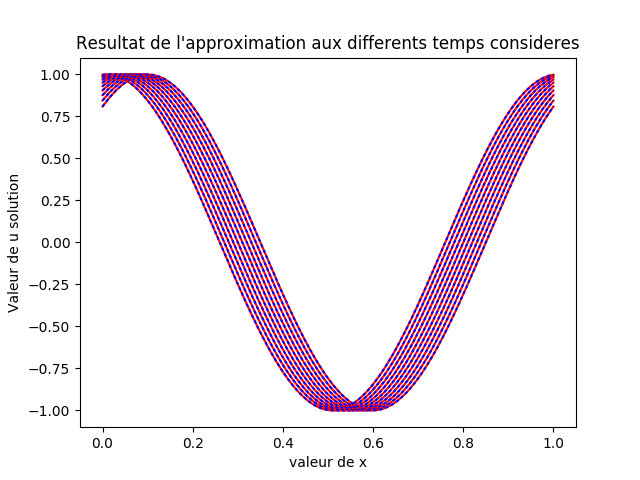
\includegraphics[scale=0.45]{1D_c1_5000_s1.png}
	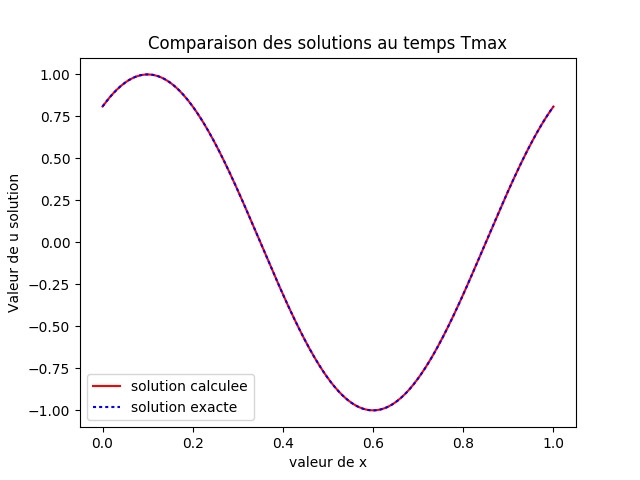
\includegraphics[scale=0.45]{Temp_max_c1_5000_s1.png}
	\caption{Approximation, discretisation de 5000 et visulation au temps max}
	\label{1D} 
	\end{figure}
Erreur max = $0.017672$
\\Deuxième condition initiale : $-\frac{2}{\pi}arctan(100(x-0.5))$
 \begin{figure}[H]
	\centering
	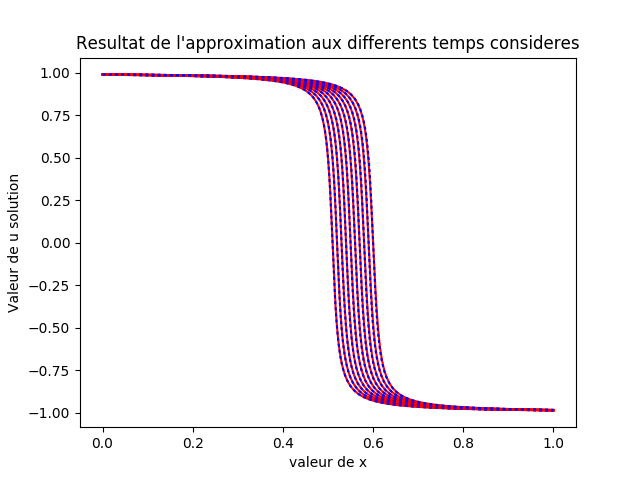
\includegraphics[scale=0.45]{1D_c1_5000_s1_init2.png}
	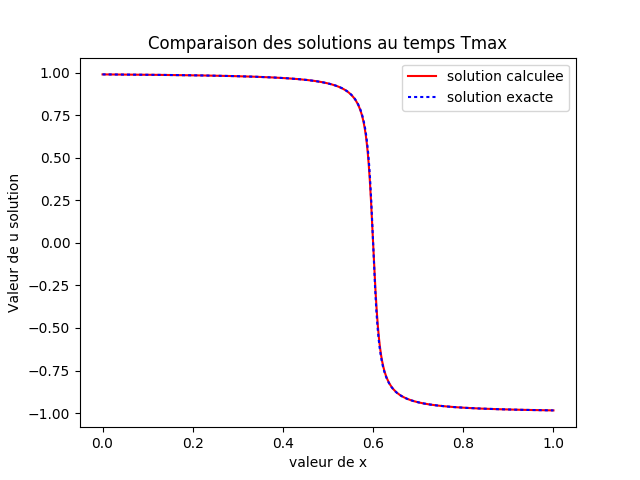
\includegraphics[scale=0.45]{Temp_max_c1_5000_s1_i2.png}
	\caption{Approximation, discretisation de 5000 et visulation au temps max}
	\label{1D} 
	\end{figure}
Erreur max = $0.337537$
\\Troisième condition initiale : $1.*(x<0.2)$
 \begin{figure}[H]
	\centering
	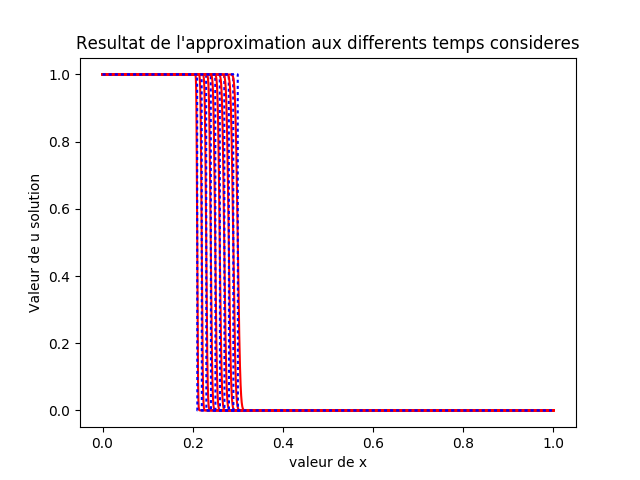
\includegraphics[scale=0.45]{1D_c1_5000_s1_init3.png}
	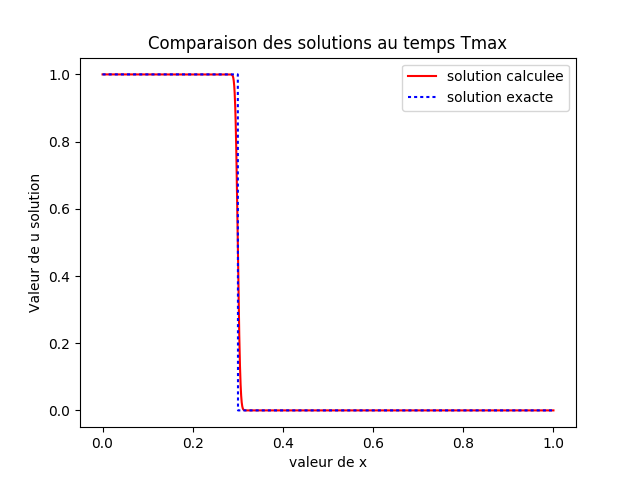
\includegraphics[scale=0.45]{Temp_max_c1_5000_s1_i3.png}
	\caption{Approximation, discretisation de 5000 et visulation au temps max}
	\label{1D} 
	\end{figure}
Erreur max = $2.261373$
\subsubsection{schéma de Richardson}

Premiére condition initiale : $cos(2 \pi x)$
 =
Erreur max = 
\\Deuxième condition initiale : $-\frac{2}{\pi}arctan(100(x-0.5))$

Erreur max =
\\Troisième condition initiale : $1.*(x<0.2)$

Erreur max = 

\subsubsection{schema de Lax Wendroff}
Premiére condition initiale : $cos(2 \pi x)$

 \begin{figure}[H]
	\centering
	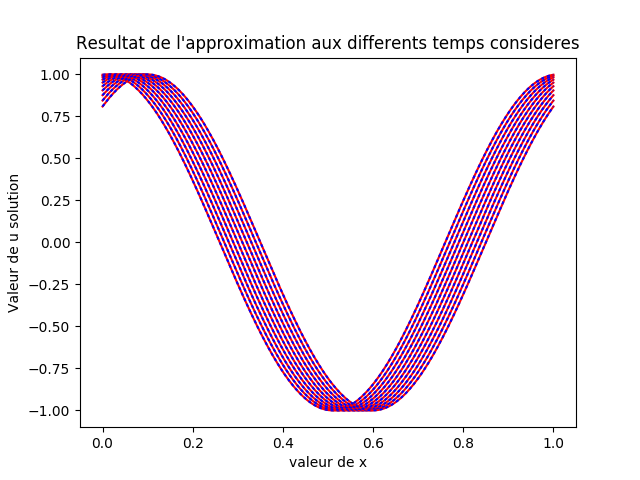
\includegraphics[scale=0.45]{1D_c1_5000.png}
	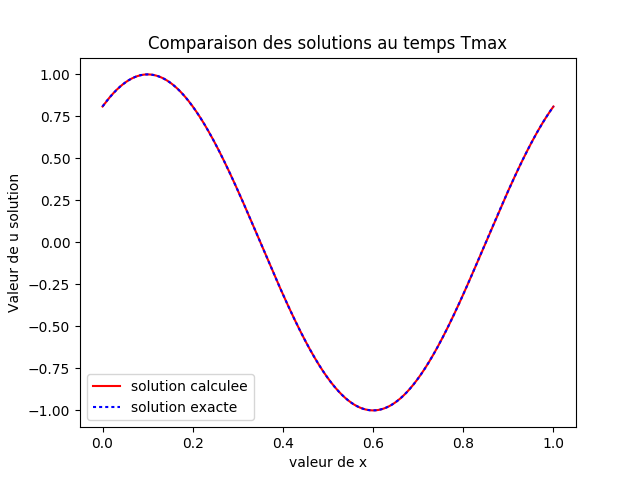
\includegraphics[scale=0.45]{Temp_max_c1_5000.png}
	\caption{Approximation, discretisation de 5000 et visulation au temps max}
	\label{1D} 
	\end{figure}
Erreur max = $0.020306$
\\Deuxième condition initiale : $-\frac{2}{\pi}arctan(100(x-0.5))$

 \begin{figure}[H]
	\centering
	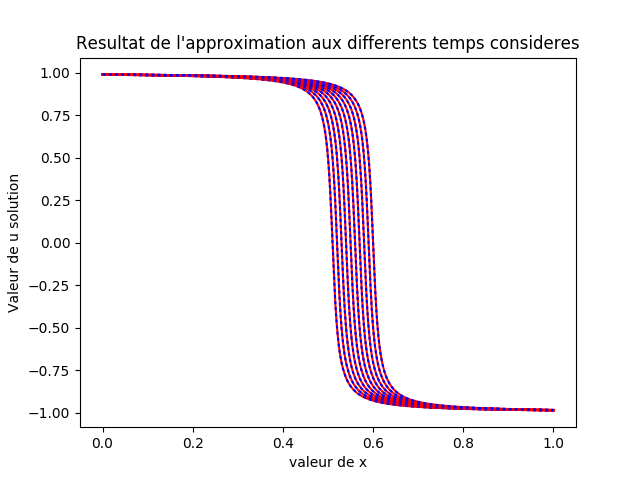
\includegraphics[scale=0.45]{1D_c1_5000_init2.png}
	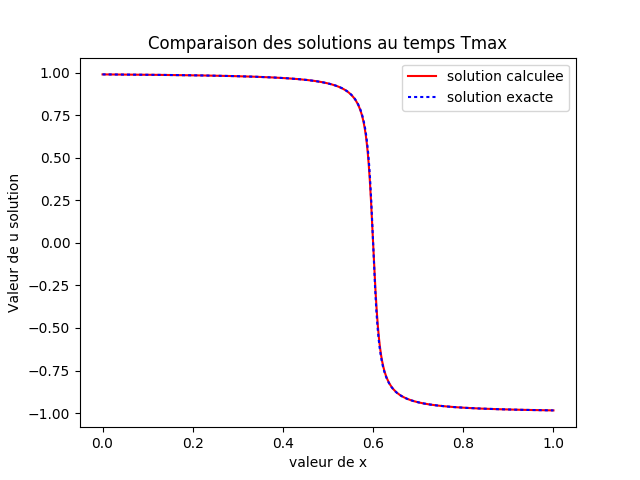
\includegraphics[scale=0.45]{Temp_max_c1_5000_s1_i2.png}
	\caption{Approximation, discretisation de 5000 et visulation au temps max}
	\label{1D}
	\end{figure}
Erreur max = $1.430819$
\\Troisième condition initiale : $1.*(x<0.2)$

 \begin{figure}[H]
	\centering
	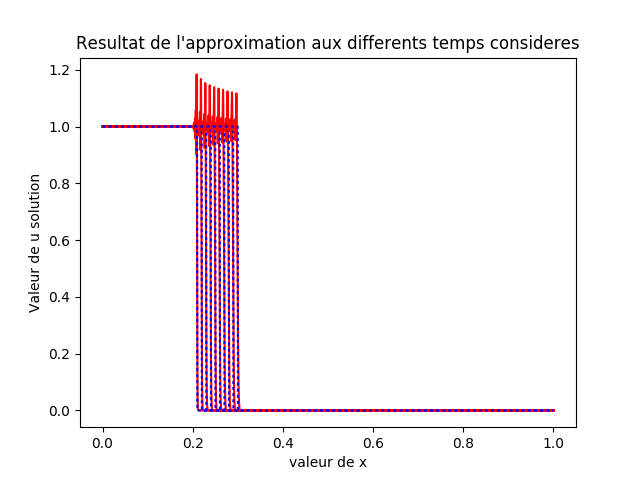
\includegraphics[scale=0.45]{1D_c1_5000_init3.png}
	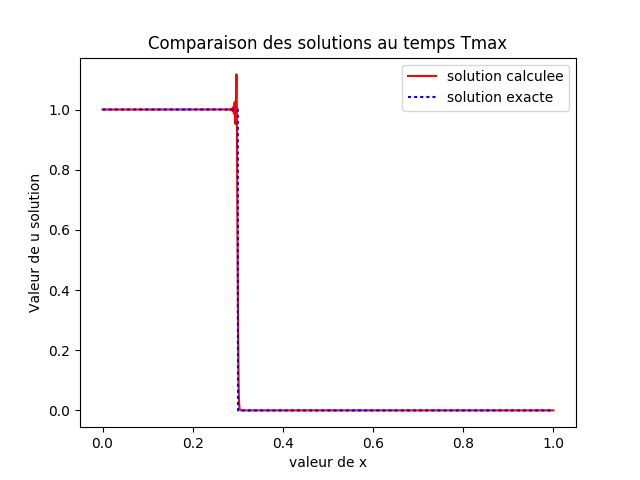
\includegraphics[scale=0.45]{Temp_max_c1_5000_init3.png}
	\caption{Approximation, discretisation de 5000 et visulation au temps max}
	\label{1D}
	\end{figure}
Erreur max = $0.000936$
\subsubsection{schéma d'Euler explicite en aval}
\subsubsection{schéma LaxFriedrichs}

\subsection{Tests de validation}
\subsubsection{Explication}
\subsection{Tests de validation}

Comme test de validation de notre méthode calcul nous avons essayé de testé le code produit pour différentes conditions initiales(voir paragraphe précédent), de plus pour savoir si l'approximation produite est bonne nous avons créer une méthode de calcul d'erreur qui représente en échelle logarithmique l'erreur entre la solution calculée et la solution exacte que nous connaissons pour toute condition initiale d'après ce que nous avons dit précédemment sur la méthode des droites caractéristiques(voir première partie).

\section{Le cas général}
\subsection{Généralisation à la dimension 2}
\noindent On cherche à généraliser le cas 1D de l'équation de transport à son problème 2D toujours dans le cas linéaire.
\\ Soit c un vecteur vitesse à deux composantes.
\\On note $c_x$ sa première composante et $c_y$ sa seconde.
On peut par exemple considérer $x$ et $y$ dans un domaine $(0,1)$.
\\Ainsi l'équation de transport en 2 dimensions est donnée par :
\\
\begin{eqnarray*}
      \left\{
        \begin{array}{llll}
            \partial_tu(t,x,y)+c.\nabla u=\partial_tu(t,x,y) +c_x\partial_xu(t,x,y)+c_y\partial_yu(t,x,y)=0
            \\ u(0,x,y)=u_0(x,y) \text{ condition initiale}
        \end{array}
    \right .
\end{eqnarray*}
\\
\\Dans le cas 1D un des schémas possible était le suivant :
\\- le schéma décentré amont et aval :
\begin{eqnarray*}
        u^{n+1}_i=u_i^n-\frac{c\Delta t}{\Delta x}({u_{i}^n-u_{i-1}^n}) \text{       , si c>0}
        \iff u^{n+1}_i=u_i^n\left(1-\frac{c\Delta t}{\Delta x}\right)+u_{i-1}^n\left(\frac{c\Delta t}{\Delta x}\right)	
        \\u^{n+1}_i=u_i^n-\frac{c\Delta t}{\Delta x}({u_{i+1}^n-u_{i}^n}) \text{       , si c<0}
        \iff u^{n+1}_i=u_i^n\left(1+\frac{c\Delta t}{\Delta x}\right)-u_{i+1}^n\left(\frac{c\Delta t}{\Delta x}\right)
\end{eqnarray*}
\\
\\Si on cherche maintenant à généraliser ce résultat pour une discrétisation 2D on obtient :
\\
\begin{center}
        \text{si c>0 : } $\displaystyle\frac{u_{i,j}^{n+1}-u_{i,j}^{n}}{\Delta t}=\frac{c_x}{\Delta x}(u_{i-1,j}^n-u_{i,j}^n)+\frac{c_y}{\Delta y}(u_{i,j-1}^n-u_{i,j}^n)$
        \\
        \text{si c<0 : }$ \displaystyle\frac{u_{i,j}^{n+1}-u_{i,j}^{n}}{\Delta t}=\frac{c_x}{\Delta x}(u_{i,j}^n-u_{i+1,j}^n)+\frac{c_y}{\Delta y}(u_{i,j}^n-u_{i,j+1}^n)$
\end{center}
On note $P_{i,j}$=$(i \Delta x,j \Delta y)$ où $i$,$j$ $\in\mathbb{Z}$, les noeuds du maillage de $\mathbb{R}^2$  $u_{i,j}$=$u(i \Delta x,j \Delta y)$ est une approximation de la solution exacte aux noeuds $P_{i,j}$ à l'instant $n\Delta t$.
\\On pourra choisir un maillage non uniforme i.e un maillage où le pas d'espace en la variable $x$ n'est pas le même que le pas d'espace en la variable $y$.
Ainsi la principale différence entre le problème 1D et le problème 2D et l'ajout de nouvelles variables qui imposent à l'inconnu u que l'on cherche à identifier d'être représenté sous forme d'une matrice ou x agit sur les lignes et y sur les colonnes.
\newpage
\subsection{Application à un exemple}
Soit le problème suivant
\begin{eqnarray*}
      \left\{
        \begin{array}{llll}
            \partial_tu(t,x,y)+c.\nabla u=\partial_tu(t,x,y) +3\partial_xu(t,x,y)+2\partial_yu(t,x,y)=0
            \\ u(0,x,y)=sin(2\pi x)sin(2\pi y) \text{ condition initiale}
            \\u(0,y,t)=u(1,y,t)
            \\u(x,0,t)=u(x,1,t)
        \end{array}
    \right .
\end{eqnarray*}
On choisit des conditions aux limites périodiques que l'on initialise connaissant la valeur de cette fonction pour cette équation qui est $u(x,y,t)=sin(2\pi (x-c_xt))sin(2\pi(y-c_yt))$, ou $c_x$=3 et $c_y=2$.
Connaissant la solution exacte on pourra par la suite calculer l'erreur entre la solution exacte et la solution approchée pour voir la pertinence du schéma utilisé et du code produit.
\\On utilise le schéma défini précédemment pour le cas 2D. On obtient alors une représentation de la solution qui est de la forme suivante :
\\\begin{figure}[H]
	\centering
	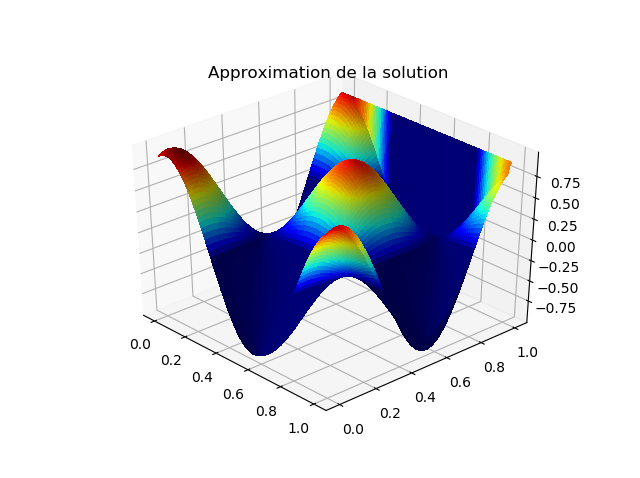
\includegraphics[scale=0.5]{Approximation_de_la_solution.png}
		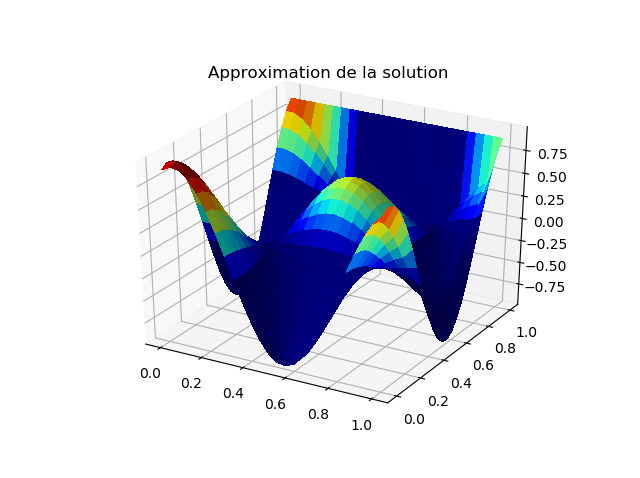
\includegraphics[scale=0.5]{Approximation_de_la_solution-1_discretisation25.png}
	\caption{$\Delta x=\Delta y$ Discrétisation par 100 et 25}
	\label{1D}
	\end{figure}

\subsection{Résolution du problème de rupture de barrage des équations de Saint Venant}
\subsubsection{Les équations de Saint-Venant}
à rédiger...
\subsubsection{Résolution du systéme d'équation de Saint Venant}
à rédiger...

\section{Bibliographie}
Livres BU : Résolution numérique des équations de Saint-Venant par la technique de projection en utilisant une méthode des volumes finis dans un maillage non structuré 

\bibliographystyle{unsrt}
\bibliography{biblio}

\end{document}


    
    